\section{Deployment}
\label{sec:deployment}
After the implementation phase, the Basilisk platform is deployed on a virtual server.
The virtual server used is provided by the IRB (Informatik Rechnerbetrieb) of the computer science department at Paderborn University.
Figure \ref{fig:vm_specs} show the specification of the VM.
The VM was configured to be powerful and to have a lot of memory and storage.

\begin{figure}[tbph]
	\centering
	\begin{tabular}{ll}
		\toprule
		\textbf{Specifications} &                             \\ \midrule
		CPUs                    & 16 cores                    \\ \midrule
		Memory                  & 128GB                       \\ \midrule
		Storage                 & 2TB                         \\ \midrule
		Operating System        & Debian GNU/Linux 11 (64bit) \\ \bottomrule
	\end{tabular}
	\caption{Specification of the virtual machine on which the platform is deployed.}
	\label{fig:vm_specs}
\end{figure}

The Basilisk platform consists of the 3 main services described in section \ref{sec:main_services}.
For the communication between these services, the platform also needs a RabbitMQ message server.
Also, a \ts{} is required as the \acl{jsts} for storing the benchmark results.
\\

For the platform to be easily manageable we decided to deploy the whole platform in Docker containers.
This has the advantage of using a single Docker Compose file for configuring the services and the network.

The individual services are compiled into jar files and the Docker build copies them into individual Docker images.
The build of the containers for the \ac{hcs} and \ac{jms} is simple and straight forward.
The container for the \ac{tbs} needs two additional configurations for the service to run.
First, the \iguana{} framework is installed inside the container.
Afterwards, the container is configured in the Docker Compose file to has access to the Docker socket of the server.
This is needed for the service to start and manage the Docker images and containers of the \tsp{} that are getting benchmarked.

The RabbitMQ message server is available as an official Docker container on \dockh{}.
For the \ac{jsts} we decided to use the Fuseki\footnote{\url{https://jena.apache.org/documentation/fuseki2/fuseki-main}} \ts{}, which also is available as a Docker container.
\\

In total the Docker Compose configuration consists of 5 containers that can be started and stopped with simple commands.
During a benchmark a sixth container is started which is running the \ts{}.
An overview of the setup is shown in figure \ref{fig:docker-setup}. 

\begin{figure}[tbph]
	\centering
	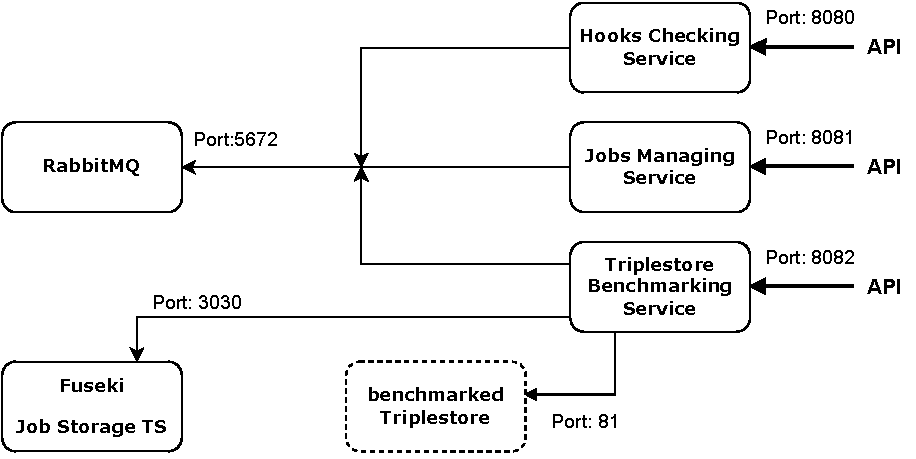
\includegraphics[width=.7\textwidth]{figures/docker-setup.pdf}
	\caption{Overview of the deployed Docker containers and used Ports.}
	\label{fig:docker-setup}
\end{figure}

The three microservices of the Basilisk platform are available through the ports 8080 (\ac{hcs}), 8081 (\ac{jms}), and 8082 (\ac{tbs}) of the host server.
RabbitMQ container is available through port 5672 and the Fuseki \ts{} which is used as the Job Storage for the benchmark results is reachable at port 3030 of the host server.
During a benchmark, the tested \ts{} is started in its own Docker container which also has port 81 published for reaching the SPARQL endpoint.